\section{Low-Entropy Analysis Methodology} \label{sec:4extension-and-compilation}
% In the preceding section, we detailed our methodology for modeling the attacker's brute-force capabilities using a set of general rules.
% This section elucidates the application of our approach to protocol modeling.
% To streamline the modeling of protocols, we extended TAMARIN's syntax by introducing new keywords that explicitly identify low-entropy keys requiring special attention within the protocol.
% 
% We also developed a compilation tool which translates the extended TAMARIN's syntax into a TAMARIN recognizable model.
% Besides this, our tool will automatically add message derivation facts by analyzing the derivation relationships between variables in the model. 

% In this section, we explain how to apply our approach to protocol modeling.
% To facilitate the modeling of protocols, we have extended \Tamarin{}'s syntax by introducing new keywords that explicitly identify low-entropy keys, which require special attention within the protocol.
% % 
% Additionally, we developed a compilation tool that translates the extended \Tamarin{} syntax into a model recognizable by \Tamarin{}.
% Furthermore, our tool automatically adds message derivation facts by analyzing the derivation relationships between variables in the model.

% To facilitate automated model verification, our Tamarin-Compilation-Tool supports the definition of search boundaries for oracle rules tailored to different protocol scenarios.
% This feature is crucial for preventing non-terminating analysis, ensuring that the verification process completes efficiently and reliably.

% In this section, we elucidate the application of our modeling approach to protocol analysis. 
In this section we describe how to apply our oracle modeling approach to analyze low-entropy keys in protocols.
To enhance the modeling of protocols using our methodology, we have devised an innovative rule syntax that serves as a superset of \Tamarin{}'s syntax. 
This new syntax incorporates several new keywords designed to identify low-entropy keys that require special attention. 
Additionally, to facilitate our new syntax, we have developed an automated low-entropy analysis tool, EntropyVerif. 
This tool integrates the key-breaking oracle discussed in the previous section, enabling attackers
to compromise low-entropy keys, thus providing a security analysis of protocols tolerant to such
keys.
To support the operation of the key-breaking oracle, our tool automatically analyzes the derivation relationships among variables within the model and generates message derivation facts. 
Finally, to ensure the automation and efficiency of the verification process, we have introduced restrictions on the oracle rules and explained these restrictions.

\subsection{ Labeled Rule Syntax } \label{sec:syntax-extension}

\Tamarin{} utilizes multiset rewriting rules to define protocol execution and adversarial behaviors.
For instance, consider the following rule demo:
\begin{flalign*}
\text{\Tterm{Rule S}}  & \text{\Tterm{endHello}} :                                      & \\
    \TLetS & \text{\Tterm{$ciphertext$ = senc("hello", $key$)}}   \\  
    \TInS & \TFacts{ \text{\TFactTerm{Share}{$key$}} }  \TEmpActFact{} \TFacts{ \text{\TFactTerm{Out}{$ciphertext$}} }
\end{flalign*}
This rule delineates a simple behavior for sending encrypted data: an entity encrypts the message "hello" using a shared $key$ and sends the $ciphertext$ to a public network.
\Tamarin{} supports local macro definitions in a rule which are defined within the \TFact{let}$ \ldots $\TFact{in} area called the let-block, where each line specifies a substitution.
In the above demo, \Tterm{$ciphertext$} in this rule will be replaced by \Tterm{senc("hello", $key$)} when the rule is executed.

To apply our methodology, we introduced a new operator ``:='' and a keyword ``\verb|`L`|''.
These syntax elements facilitate the identification and labeling of low-entropy variables.
In the extended syntax, as depicted in the following rule, the low-entropy label for the variable is defined within the let block.
\begin{flalign*}
    \text{\Tterm{Rule S}}   & \text{\Tterm{endHello}} :                         & \\
    \TLetS                  & \text{\Tterm{$key$ := `L`}}                         \\  
                            & \text{\Tterm{$ciphertext$ = senc("hello", $key$)}}    \\  
    \TInS                   & \TFacts{ \text{\TFactTerm{Share}{$key$}} }  \TEmpActFact{} \TFacts{ \text{ \TFactTerm{Out}{$ciphertext$}} }
\end{flalign*}
Here, the label ``\verb|`L`|'' on the right side of ``:='' signifies that the variable $key$ on the left possesses a low entropy.
This label will be recognized by EntropyVerif and translated into a fact $\text{\TFact{EntropyLow}}(key)$ added to the right-hand side of the rule.

\subsection{ Design of EntropyVerif }

\begin{figure}[t]
    \centering
    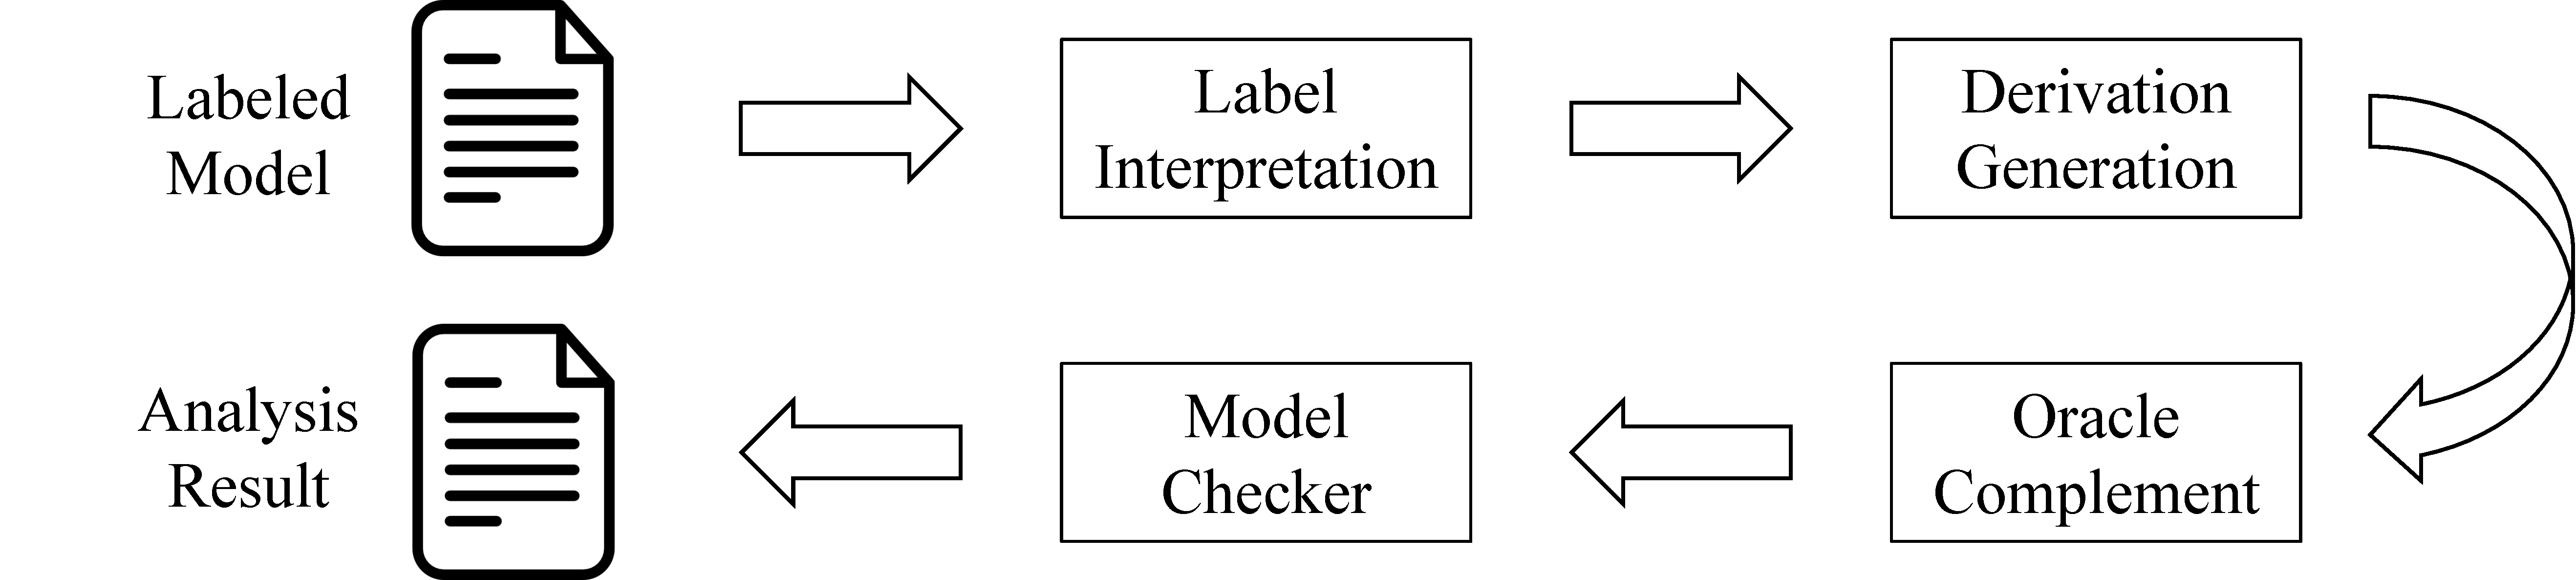
\includegraphics[width=\columnwidth]{img/tool}
    \caption{Architecture of EntropyVerif}
    \label{fig:design-of-compilation-tool}
\end{figure}

EntropyVerif is an extension of \Tamarin{} and 
supports low-entropy labeled protocol models and integrates an adversarial model with the capability to brute-force low-entropy keys.
As shown in \autoref{fig:design-of-compilation-tool}, EntropyVerif contains 4 modules:
\begin{enumerate}[leftmargin=*]
    \item \textbf{Label Interpretation:} This module is responsible for identifying and parsing the low-entropy labels of terms, subsequently generating the \TFact{EntropyLow} facts.
    \item \textbf{Derivation Generation:} This module analyzes the message derivation relationships between terms in symbolic models and generates \TFact{MDerive} facts.
    \item \textbf{Oracle Complement:} This module adds the key-breaking oracle to the model and incorporates reasonable restrictions to prevent automated verification from entering a non-terminating state.
    \item \textbf{Verifier:} This module conducts a formal analysis of the model generated by preceding modules. 
\end{enumerate}

We successfully implemented Label Interpretation, Derivation Generation, and Oracle Complement modules, while employing \Tamarin{} as the Verifier in our study.

\subsection{ Analysis Details }

\begin{table}[t]
    \centering
    \caption{Notation used throughout the methodology.}
    \label{tab:notation}
    \renewcommand{\arraystretch}{1.15}
    \small
    \begin{tabular}{@{}ll@{}}
    \toprule
    Symbol & Meaning \\
    \midrule
    $\mathsf{sub}(t)$           & Syntactic subterms of $t$ \\
    $\mathsf{atoms}(t)$         & Atomic terms occurring in $t$ \\
    $\mathsf{vars}(t)$          & Atomic terms of $t$ that are not constants \\
    $\mathsf{const}(T)$         & Constants and public names in $T$ \\
    $\mathsf{terms}(F)$         & Terms occurring as arguments of the facts in $F$ \\
    $df_\mathcal{P}$            & Derivation facts emitted from protocol rules \\
    $df_\mathcal{O}$            & Oracle-side closure of derivation facts \\
    $dm_\mathcal{A}$            & Messages derivable by the Dolev--Yao attacker \\
    \bottomrule
    \end{tabular}
\end{table}

% All terms in the translated multiset rewriting rules remain consistent with their original form.
To describe the translation we use the operations listed in \autoref{tab:notation}, all of which
are defined on sets.
Throughout, a term is \emph{atomic} if it is a variable, a fresh name, or a public constant. Every
other term has the form $f(t_1,\ldots,t_n)$ for a function symbol $f$ declared in the model.

For a term $t$, $\mathsf{sub}(t)$ is the set of syntactic subterms of $t$:
\[
    \mathsf{sub}(t) =
    \begin{cases}
        \{t\} & \text{$t$ atomic,} \\[2pt]
        \{t\} \cup \bigcup_{i=1}^{n} \mathsf{sub}(t_i) & \text{$t = f(t_1,\ldots,t_n)$.}
    \end{cases}
\]
The definition is purely syntactic. It does not close the set under the equational theory, and it
does not refer to what an attacker is able to derive. Both of those are left to \Tamarin{} during
verification.

Dually, $\mathsf{atoms}(t)$ is the set of atomic terms out of which $t$ is built:
\[
    \mathsf{atoms}(t) =
    \begin{cases}
        \{t\} & \text{$t$ atomic,} \\[2pt]
        \bigcup_{i=1}^{n} \mathsf{atoms}(t_i) & \text{$t = f(t_1,\ldots,t_n)$.}
    \end{cases}
\]
Reading $t$ as a tree, $\mathsf{sub}(t)$ collects every node and $\mathsf{atoms}(t)$ collects the
leaves. Both operations are lifted to a set of terms $T$ by taking the union over its elements, so
that $\mathsf{sub}(T) = \bigcup_{t \in T} \mathsf{sub}(t)$, and likewise for $\mathsf{atoms}$.

We write $\mathsf{const}(T)$ for the subset of $T$ consisting of constants and public names, and
abbreviate $\mathsf{vars}(t) = \mathsf{atoms}(t) \setminus \mathsf{const}(\mathsf{atoms}(t))$ for
the non-constant leaves of $t$. For a collection of facts $F$, $\mathsf{terms}(F)$ is the set of
terms occurring as arguments of those facts.

As in \Tamarin{}, the two sides of a multiset rewriting rule are multisets of facts, written
$[F_L] \rightarrow [F_R]$, and $\uplus$ denotes multiset union. Every other collection in this
section is a set. A fact argument must be a single term, so wherever a set of terms has to be
passed to a fact we arrange it in a fixed order and pass the resulting tuple, written $\langle
\cdot \rangle$. That order belongs to the encoding and carries no meaning.

% 在上述的notations的基础之上，我们将解释我们的工具如何验证低熵标记的协议模型
Based on the aforementioned notations, we explain how EntropyVerif verifies protocol models with low-entropy labels.

% 标签翻译 给低熵term的标记，准确来说并不属于多重集重写系统，引入它是为了方便在现有的规则中标注出低熵term。对于规则$F_L \rightarrow F_R$，我们使用$T_{Low}$代表这条规则中被标记的低熵term，$T_{Low} \subseteq \varepsilon(\tau(F_L)) \circ \varepsilon(\tau(F_R))$。我们定义低熵标签被翻译的规则如下：
% 其中，为了简洁，我们使用$\text{LE}(T_{Low})$来代表一个序列，that consists of fact $\text{\TFact{EntropyLow}}(t)$ for each term $t$ in $T_{Low}$.
\noindent
\textbf{Label Interpretation:} 
Labels of low-entropy terms are not inherently part of the multiset rewriting system. 
It is introduced to facilitate the identification of such terms within existing rules.
For a given rule $[F_L] \rightarrow [F_R]$, $T_{Low}$ denotes the set of low-entropy terms labeled
in the rule, where $T_{Low} \subseteq \mathsf{sub}(\mathsf{terms}(F_L)) \cup
\mathsf{sub}(\mathsf{terms}(F_R))$.
The translated version of such a rule with low-entropy labels is shown as follows:
\[
    [F_L] \rightarrow [F_R \uplus \text{\textsf{LE}}(T_{Low})]
\]
where, for brevity, we write $\text{\textsf{LE}}(T_{Low})$ for the multiset $\{\,
\text{\TFact{EntropyLow}}(t) \mid t \in T_{Low} \,\}$.

% 我们以\autoref{sec:syntax-extension}中低熵标记的规则为例，该规则中在Label Interpretation模块中会被翻译为如下的rule：
We take the rule labeled with low entropy in \autoref{sec:syntax-extension} as an example. 
In the Label Interpretation, it will be translated into the following rule:
\begin{flalign*}
    \text{\Tterm{Rule S}}   & \text{\Tterm{endHello}} :                         & \\
    \TLetS                  & \text{\Tterm{$ciphertext$ = senc("hello", $key$)}}    \\  
    \TInS                   & \TFacts{ \text{\TFactTerm{Share}{$key$}} }          \\
    \TEmpActFact{} \hspace{0.2em}& \TFacts{ \text{ \TFactTerm{Out}{$ciphertext$} }, \text{ \TFactTerm{EntropyLow}{$key$} }  }
\end{flalign*}

% 派生生成 对于规则$[F_L] \rightarrow [F_R]$，$\tau(F_R)$代表了这条规则执行之后存在的term，而$\varepsilon(\tau(F_L))$则代表了这条规则所有的已知term。因此，我们可以使用$\tau(F_R) \setminus \varepsilon(\tau(F_L))$来表示规则执行所派生出的新term。我们定义添加消息派生事实之后的规则如下：
% 这里我们使用$\text{\textsf{MD}}(T)$来表示消息派生事实序列，其中序列T的每个元素都是一个term的消息派生事实。对于单个term $t$，$\rho(t) \setminus c(\rho(t)) $ 包含了构建$t$所需的所有变量term。
% 这里我们使用$\text{\textsf{MD}}(T)$来表示来表示使用序列T中每个term作为计算结果的消息派生事实。对于单个term $t$，$\rho(t) \setminus c(\rho(t)) $ 包含了构建$t$所需的所有变量term。那么$\text{\textsf{MD}}(T)$可以被定义为$\text{\TFact{MDerive}(\langle \rho(t) \setminus c(\rho(t)) \rangle, t)}$ for each term $t$ in $T$。
\noindent
\textbf{Derivation Generation:} 
Given the rule $[F_L] \rightarrow [F_R]$, $\mathsf{terms}(F_R)$ denotes the terms present within
the rule after executing, whereas $\mathsf{sub}(\mathsf{terms}(F_L))$ represents all possibly
accessible terms before the execution.

Thus, $\mathsf{terms}(F_R) \setminus \mathsf{sub}(\mathsf{terms}(F_L))$ can be used to represent
the new terms derived during the execution of the rule.
We define the rules incorporating message derivation facts as follows:
\[
    [F_L] \rightarrow [F_R \uplus \text{\textsf{MD}}(\mathsf{terms}(F_R) \setminus \mathsf{sub}(\mathsf{terms}(F_L)))]
\]
Here, $\text{\textsf{MD}}(T)$ denotes the set of message derivation facts.
For an individual term $t$, $\mathsf{vars}(t)$ contains the non-constant leaves needed to
construct it.
Hence $\text{\textsf{MD}}(T)$ can be defined as
$\{\, \text{\TFact{MDerive}}(\langle \mathsf{vars}(t) \rangle, t) \mid t \in T \,\}$.

We take the rule in \autoref{sec:syntax-extension} as an example as well. 
A message derivation fact will be added to the right-hand side of the rule as follows:
\begin{flalign*}
    \text{\Tterm{Rule S}}   & \text{\Tterm{endHello}} :                         & \\
    \TLetS                  & \text{\Tterm{$ciphertext$ = senc("hello", $key$)}}    \\  
    \TInS                   & \TFacts{ \text{\TFactTerm{Share}{$key$}} }          \\
    \TEmpActFact{} \hspace{0.2em}& \TFacts{ \text{ \TFactTerm{Out}{$ciphertext$} }, \text{ \TFactTerm{EntropyLow}{$key$} }, \\
                            & \hspace{5em} \text{ \TFactTerm{MDerive}{$key$, $ciphertext$} }}
\end{flalign*}


% \subsection{An illustrative example}

% \begin{figure}[htbp]
%     \centering
%     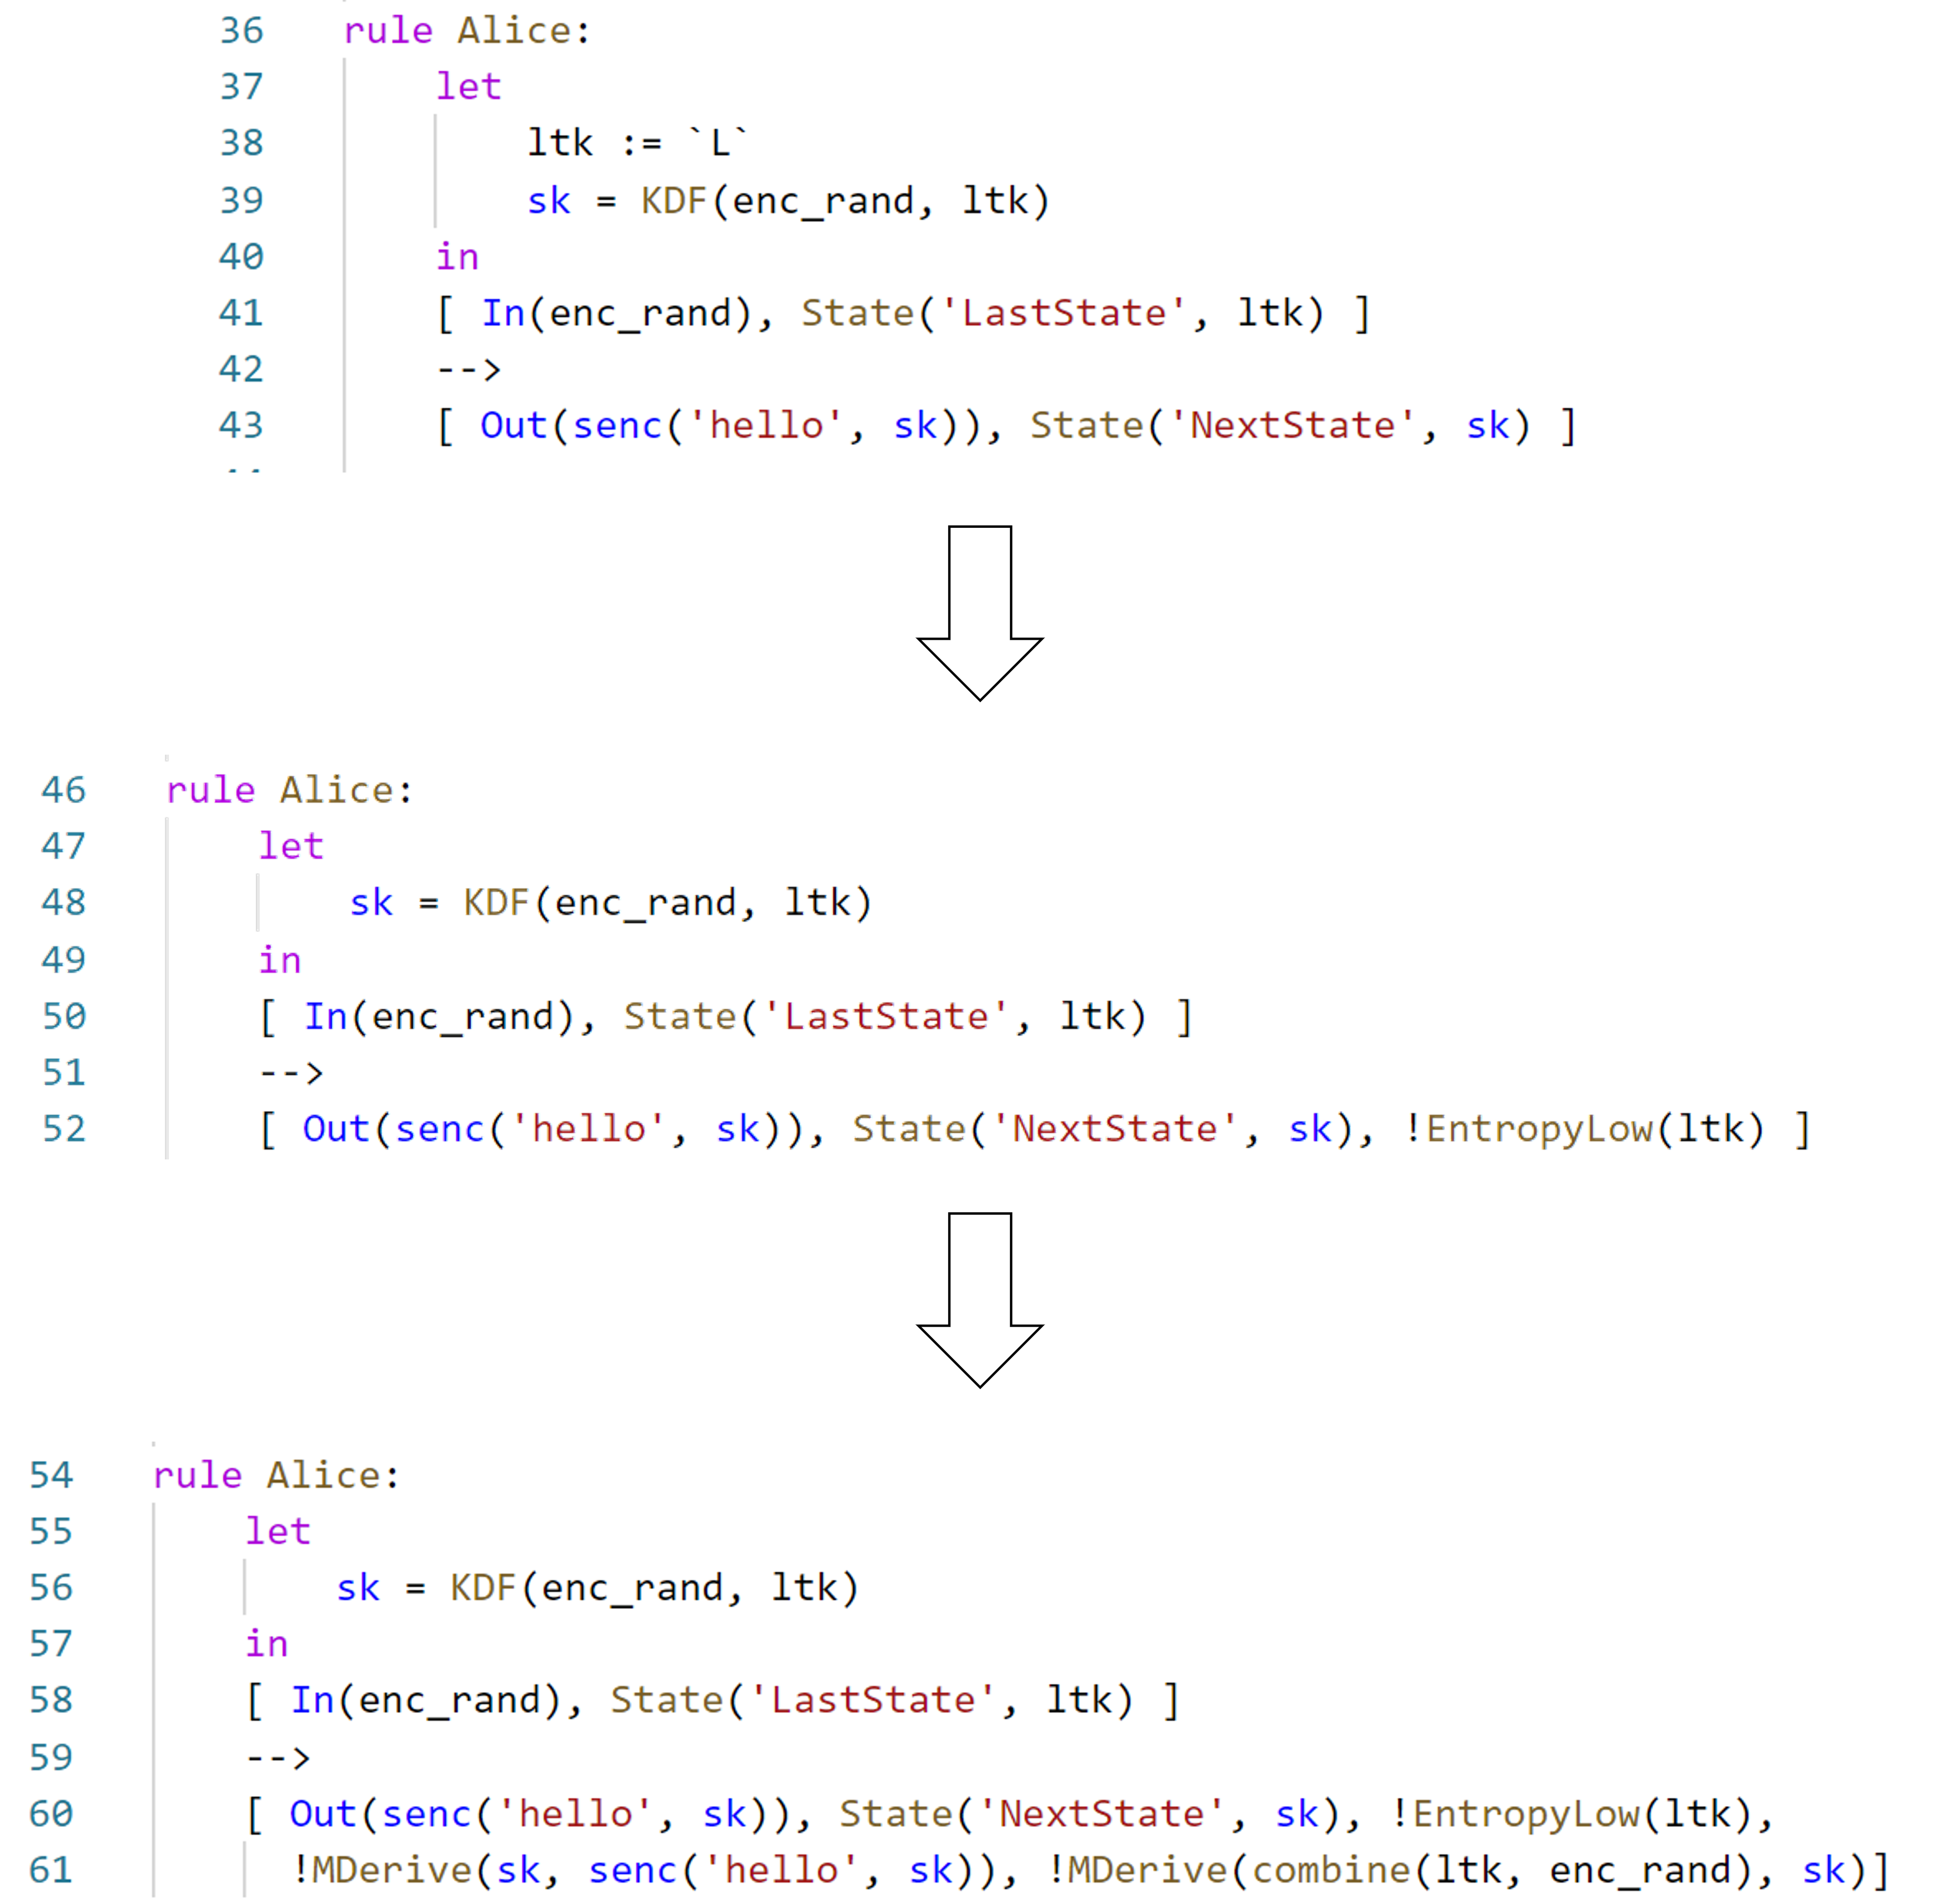
\includegraphics[width=\columnwidth]{img/rule_compile}
%     \caption{Rule Comp}
%     \label{fig:rule-compile}
% \end{figure}

% % \autoref{fig:rule-compile}展示一个
% \autoref{fig:rule-compile} 

% \subsection{ Restriction of  Oracle Rules }

% 尽管上述的工作使得oracle具备了运行的条件，然而，为了验证工作的自动化和效率，避免系统进入无法终止的状态，我们需要为oracle的rule添加一些限制。前文我们使用$\rho(t) \setminus c(\rho(t))$来表示参与$t$ 构造的所有变量。通过考虑$\rho(t) \setminus c(\rho(t))$，我们可以给出一个定义：
% 如果t可以被Oracle破解，那么oracle rule的执行次数一定小于等于$\rho(t) \setminus c(\rho(t))$的中的元素个数。
\noindent
\textbf{Oracle Complement:} 
The Oracle Complement module adds the key-breaking oracle to protocol models and generates appropriate restrictions.
Despite the aforementioned work enabling the oracle to operate, additional restrictions on the oracle's rules are necessary to ensure automation, and efficiency, and to prevent the system from entering a non-terminating state.

For a given term $t$, $\mathsf{vars}(t)$ contains all variables required to construct it.
Since $\mathsf{vars}(t)$ is finite and each execution of an oracle rule consumes one of its
elements, if $t$ can be compromised by the oracle then the oracle rule is executed at most
$|\mathsf{vars}(t)|$ times.
So in the Oracle Complement module, we reserved a verification option to dynamically restrict the number of times the oracle rule can be executed.

\noindent
\textbf{Verifier:} 
In EntropyVerif, \Tamarin{} is employed as the Verifier to analyze the model generated by the aforementioned modules.
The last module, Oracle Complement, outputs the generated model to the Verifier module in a format compatible with \Tamarin{}. 
The Verifier verifies whether the security properties in the protocol are satisfied and outputs the results to an analysis results file.
